\documentclass[conference]{IEEEtran}
\IEEEoverridecommandlockouts
% The preceding line is only needed to identify funding in the first footnote. If that is unneeded, please comment it out.


\usepackage{scalerel}
\usepackage{tikz}
\usetikzlibrary{svg.path}

\definecolor{orcidlogocol}{HTML}{A6CE39}
\tikzset{
  orcidlogo/.pic={
    \fill[orcidlogocol] svg{M256,128c0,70.7-57.3,128-128,128C57.3,256,0,198.7,0,128C0,57.3,57.3,0,128,0C198.7,0,256,57.3,256,128z};
    \fill[white] svg{M86.3,186.2H70.9V79.1h15.4v48.4V186.2z}
                 svg{M108.9,79.1h41.6c39.6,0,57,28.3,57,53.6c0,27.5-21.5,53.6-56.8,53.6h-41.8V79.1z M124.3,172.4h24.5c34.9,0,42.9-26.5,42.9-39.7c0-21.5-13.7-39.7-43.7-39.7h-23.7V172.4z}
                 svg{M88.7,56.8c0,5.5-4.5,10.1-10.1,10.1c-5.6,0-10.1-4.6-10.1-10.1c0-5.6,4.5-10.1,10.1-10.1C84.2,46.7,88.7,51.3,88.7,56.8z};
  }
}

\newcommand\orcidicon[1]{\href{https://orcid.org/#1}{\mbox{\scalerel*{

\begin{tikzpicture}[yscale=-1,transform shape]
\pic{orcidlogo};
\end{tikzpicture}
}{|}}}}

\usepackage{hyperref} %<--- Load after everything else




\usepackage{cite}
\usepackage{amsmath,amssymb,amsfonts}
\usepackage{algorithmic}
\usepackage{graphicx}
\usepackage{textcomp}
\usepackage{xcolor}
\def\BibTeX{{\rm B\kern-.05em{\sc i\kern-.025em b}\kern-.08em
    T\kern-.1667em\lower.7ex\hbox{E}\kern-.125emX}}
\begin{document}

\title{Dataset: BLE RSS dataset for fingerprinting radio map calibration}

\author{\IEEEauthorblockN{Marcin Kolakowski \orcidicon{0000-0003-0068-8784}}
\IEEEauthorblockA{\textit{Institute of Radioelectronics and Multimedia Technology} \\
\textit{Warsaw University of Technology}\\
Warsaw, Poland \\
m.kolakowski@ire.pw.edu.pl}

}

\maketitle

\begin{abstract}
This document describes a dataset of Bluetooth Low Energy signals strengths measured in a fully furnished fla.  The dataset was originally used in the study concerning RSS-fingerprinting--based indoor positioning systems. The data were gathered using a hybrid BLE-UWB localization system, which was installed in the apartment and a mobile robotic platform equipped for a LiDAR. The dataset comprises power measurement results and LiDAR scans performed in 4104 points. The scans used for initial environment mapping and power levels registered for two test scenarios are also attached. 
The set contains both raw and preprocessed measurement data. The Python code for raw data loading is supplied.
\end{abstract}

\begin{IEEEkeywords}
BLE, fingerprinting, positioning, RSS
\end{IEEEkeywords}

\section{Introduction}
This dataset contains Received Signal Strengths (RSS) of the Bluetooth Low Energy signals registered in a fully furnished apartment. The data were used to assess the effectiveness of radio map calibration methods in a yet unpublished paper.

The dataset consists of three parts:
\begin{itemize}
\item SLAM measurements - 79 stationary scans gathered in an apartment,
\item RSS calibration dataset - 4104 fingerprints,
\item test dataset - RSS measurements performed in two test scenarios - robot and walking person localization.
\end{itemize}

\section{Files}
The dataset consists of files containing measurement results, measurement locations and a Python script:
\begin{itemize}
\item \texttt{x.log} - where $x=1..57$ - output log files containing CIR and distance measurement results,
\item \texttt{anchors.csv} - x-y coordinates of the transmitter (referenced as an anchor),
\item \texttt{tags.csv} - x-y coordinates of the receiver (referenced as a tag),
\item \texttt{pairs.csv} - list of anchor-tag location pairs for which the measurements were performed,
\item \texttt{labels.csv} - LOS/NLOS labels assigned to the measurement results in paper \cite{b1},
\item \texttt{loadCIR.py} - python script decoding the log file and loading CIR and ranging measurement results.
\end{itemize} 


\section{Measurements description}

The measurements were performed using the localization system described in \cite{b1}. The layout of the apartment and the loactions of the anchors are presented in Fig.\ref{plan}.

\begin{figure}[h]
\centerline{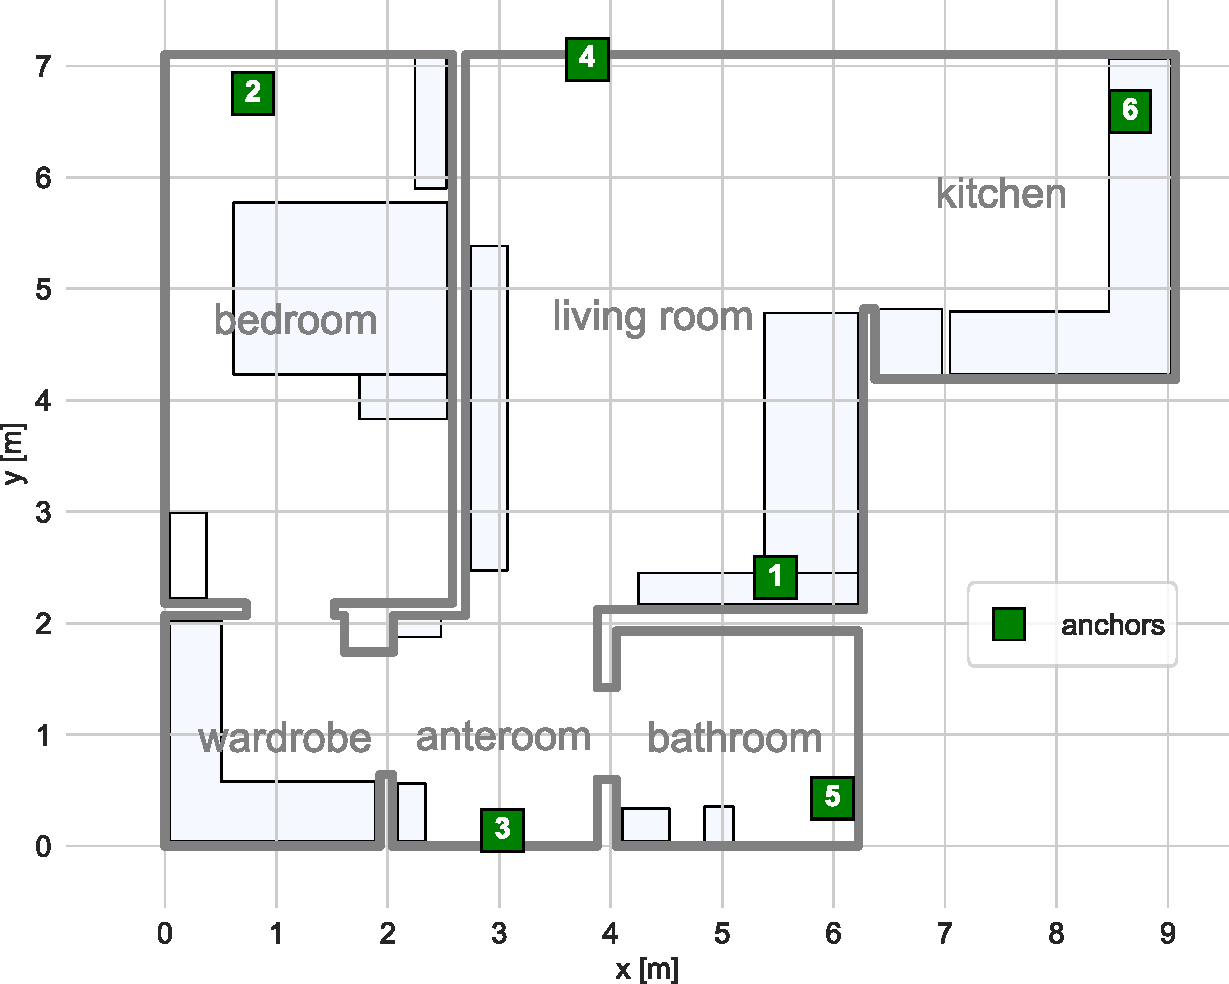
\includegraphics[width=\columnwidth]{figs/layout}}
\caption{Measurement environment with measurement locations and significant objects obstructing the path between the devices marked.}
\label{plan}
\end{figure}

The system infrastructure used in the study comprised six anchors, distributed among the apartment. The used anchors are equipped with two Laird BL652 modules with external antennas of perpendicular polarization. In the system, the tag transmits BLE packets five times per second in three advertisement channels. The anchors periodically switch the reception channels and measure the power of the received signals. The results from both modules are averaged and sent to a localization server, which stores them in a database for future processing. The measurement results were gathered using a robotic platform, which is presented in Fig.\ref{fig:robot}.

\begin{figure}[h]
\centering
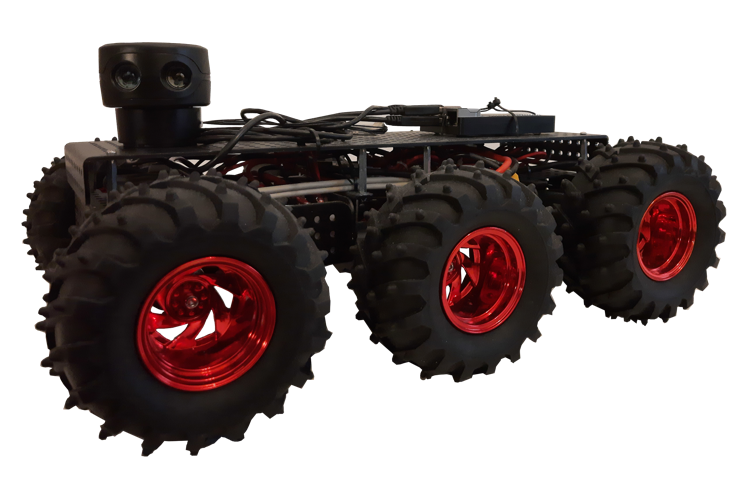
\includegraphics[width=0.8\columnwidth]{figs/robot}
\caption{\label{fig:robot}The mobile platform used in the study.}
\end{figure}


The platform was based on the Dagu Wild Thumper 6WD chassis and was controlled with a specially developed Python-based controller running on Raspberry Pi 4. The code for the controller and the PC applications used to gather the LiDAR results can be found at \cite{c2}.  The odometry measurements were performed by estimating the traveled distance and rotation angle through multiplying the elapsed time by the linear and rotation speed respectively.

The platform was equipped with a Scanse Sweep LiDAR, which is a discontinued 360 degree range sensor. During the study, the LiDAR was set to collect scans with a 2~Hz rate.

The system tag was attached at the middle the robot on a one meter long wooden pole, which placed it at the height of 1.3 m. Such height is close to a tag worn on a lanyard and ensures that low furniture pieces such as bed frames, couches or tables won't negatively impact the RSS measurement results.




\section{Licence and attribution}

The dataset is licensed under \textit{Creative Commons Attribution 4.0 International} license. The actual citation data can be found in the metadata on Zenodo or Readme file on Github.




\begin{thebibliography}{00} 
\bibitem{b1} J. Kolakowski, V. Djaja-Josko, M. Kolakowski, and K. Broczek, “UWB/BLE Tracking System for Elderly People Monitoring,” Sensors, vol. 20, no. 6, p. 1574, Mar. 2020, doi: 10.3390/s20061574.
\bibitem{b2} Marcin Kolakowski, Simple Raspberry Pi, Python based controlled for a robotic platform. 2021. Accessed: Aug. 12, 2021. [Online]. Available: https://github.com/marckolak/wtController


\end{thebibliography}
\vspace{12pt}
\color{red}

\end{document}
